\chapter{Telegestione E-Pro}
\label{capitolo6}
\thispagestyle{empty}
In questo capitolo analizzeremo quella parte di software, trascurata nel capitolo precedente, che riguarda la comunicazione tra il software di telegestione e il server JBoss. In particolare questo tipo di comunicazione non riguarda altro che l'implementazione di un protocollo di comunicazione tra i due moduli.
\section{Il protocollo di comunicazione}
Questo tipo di protocollo in realtà non è altro che lo scambio di stringhe di messaggi tra i moduli JBoss e il software \texttt{Telegestore}, e quindi la struttura è molto semplice; argomento più complesso invece è la comunicazione tra i due software che avviene tramite due canali diversi di comunicazione. Questa decisione è stata presa in quanto le  risposte da parte di una centrale telegestita risultano essere più lente rispetto al normale utilizzo di un qualsiasi software, utilizzando due canali di comunicazione è possibile disaccoppiare la comunicazione ed evitare il blocco del software. Sul primo canale si inviano i comandi al software di telegestione il quale risponderà immediatamente tramite un meccanismo di \emph{request-replay} in modo da restituire un feedback immediato all'operatore. Sul secondo canale, invece, si sfrutta un meccanismo di \emph{publish-subscribe} dove il \texttt{Telegestore} è colui che pubblica i contenuti mentre il JBoss è in ascolto, su questo canale vengono trasmesse tutte le informazioni riguardanti la centrale telegestita come lo stato di partizioni, di zone o l'avvenuta esecuzione di un comando. Il grafico di \fname{fig:teleJboss} mostra la comunicazione tra i software.
\begin{figure}
	\centering
	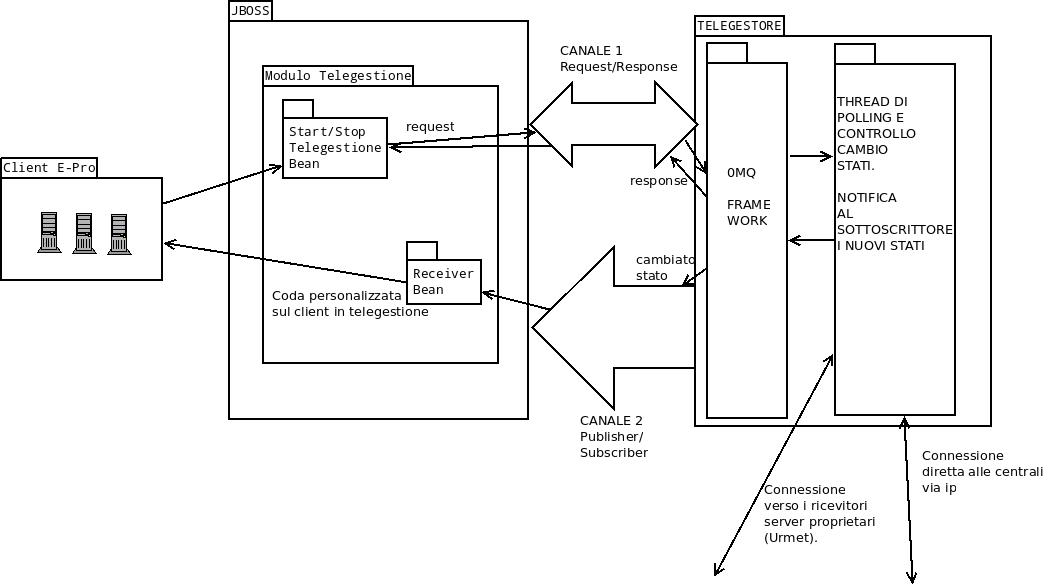
\includegraphics[width=\linewidth]{pictures/telejboss.jpeg}
	\caption{Schema di comunicazione della telegestione}\label{fig:teleJboss}
\end{figure}
\subsection{Il primo canale di comunicazione}
Il primo canale di comunicazione serve per svolgere tre compiti il primo è attivare la telegestione, il secondo disattivarla ed il terzo inviare i comandi da eseguire.
\subsubsection{La struttura del pacchetto}
La struttura del pacchetto è relativamente semplice, essa è composta da una serie di campi separati dal carattere '';'', il pacchetto è così formato:
\begin{center}
	$$ce\_id;COD;dati$$
\end{center}
\begin{description}
	\item[ce\_id:] questo campo contiene il codice identificativo della centrale;
	\item[COD:] questo campo è un codice che identifica il tipo di pacchetto e di conseguenza l'operazione da eseguire sulla centrale specificata;
	\item[dati:] questo campo ha una lunghezza variabile da 0 a 3 campi
\end{description}
Questi sono i pacchetti che il modulo eseguito sul server JBoss invia al software Telegestore, quest'ultimo risponde inviando lo stesso pacchetto ma con nel campo dati il valore \emph{OK} in caso di successo e \emph{KO} in caso di fallimento.
\subsubsection{I tipi di pacchetto}
I pacchetti che il modulo eseguito sul JBoss può inviare sono di tre tipi, il pacchetto per cominciare la telegestione, il pacchetto per interromperla e il pacchetto per eseguire il comando.\\
Il primo pacchetto di avvio della telegestione è così formattato:
$$ce\_id;AVVIO$$
quando il server lato Telegestore riceve questo comando crea un istanza di \texttt{Centrale} e ne invoca il metodo \texttt{Start} in caso tutto vada a buon fine il Telegestore risponde con il pacchetto:
$$ce\_id;AVVIO;OK$$
in caso di problemi nell'avvio della telegestione il server risponde con il messaggio:
$$ce\_id;AVVIO;KO$$
Il pacchetto di fine telegestione è simile al precedente cambia unicamente il codice comando ed il campo dati è vuoto, il pacchetto generale è:
$$ce\_id;FINE$$
Il server che riceve il messaggio invoca il metodo \texttt{Stop} sulla centrale telegestita e risponde con il messaggio:
$$ce\_id;FINE;OK$$
Il pacchetto per l'invio dei comandi contiene invece un campo dati con lunghezza diverso da 0 e il messaggio inviato è così composto:
$$ce\_id;COM;tipo;numero;comando$$
in questo caso il campo \texttt{tipo} indica il tipo di elemento sul quale applicare il comando, esso si distingue in partizione oppure zona; il campo \texttt{numero} indica il numero dell'elemento sul quale il comando deve essere eseguito, ed infine il campo \texttt{comando} indica il tipo di azione da intraprendere in base al tipo, il valore \emph{1} indica l'inserimento di una partizione oppure l'inclusione di una zona; il valore \emph{2} indica invece il disinserimento della partizione o l'esclusione della zona.\\
Il software di telegestione risponde a questo comando inserenderlo nella lista dei comandi da eseguire ed inviando il messaggio:
$$ce\_id;COM;OK$$
\subsubsection{La connessione}
La connessione avviene tramite l'utilizzo del framework ZeroMQ\cite{zmq} il quale in questo caso implementa un meccanismo di request-replay ovvero il client, il modulo JBoss, invia al server, il software Telegestore, un messaggio; il framework si preoccupa di far in modo che il messaggio arrivi a destinazione correttamente ed effettua eventuali conversioni nel tipo di dato. In questo tipo di paradigma il client non può inviare altri messaggi fino a quando il server non risponde allla prima richiesta. Questo meccanismo permette una sincronia di comunicazione tra i due software e ci permette di rispondere sempre all'ultima richiesta effettuata. In \fname{fig:contteljboss} vediamo come i due software si scambiano i messaggi.
\begin{figure}
	\centering
	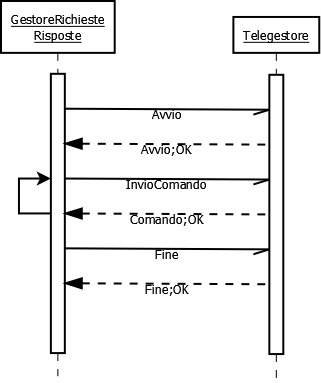
\includegraphics[width=0.5\linewidth]{pictures/congesttele.png}
	\caption{Scambio di messaggi sul canale request-replay}\label{fig:contteljboss}
\end{figure}
Un particolare di questo tipo di meccanismo è che il client risulta bloccato fino a quando non riceve una risposta e questo, in caso di invio di un comando richiederebbe diverso tempo se dovessimo aspettare l'esecuzione di tale comando sulla centrale. Per questo motivo si è deciso di inviare la conferma del comando non appena esso è stato preso in carico dal softwaare di telegestione e di utilizzare un secondo canale di comunicazione per segnalare l'avvenuta esecuzione del comando sulla centrale.
\subsection{Il secondo canale di comunicazione}
Il secondo canale di comunicazione è utilizzato per inviare al modulo in esecuzione sul JBoss gli esiti dei comandi ed eventuali variazioni degli stati degli elementi sulle centrali. Questo tipo di comunicazione avviene tramite un meccanismo di \emph{publish-subscribe} dove il Telegestore è colui che pubblica mentre il modulo JBoss si occupa di ricevere gli eventi delle centrali telegestite.
\subsubsection{La struttura del pacchetto}
I pacchetti utilizzati per lo scambio di informazioni sul secondo canale di comunicazione sono di due tipi, il primo serve per scambiare informazioni riguardo lo stato degli elementi della centrale di allarme ed è composto dai seguenti elementi:
$$ce\_id;tipo;numero;n1;n2;n3$$
nei quali gli elementi sono tutti valori numerici, in particolare il \texttt{ce\_id} serve ad individuare la centrale da cui arriva l'informazione, \texttt{tipo} è un valore numerico che serve ad indicare se si tratta di informazioni riguardanti la centrale, una partizione o una zona, il \texttt{numero} identifica il numero dell'elemento ed infine i valori \texttt{n1}, \texttt{n2} e \texttt{n3} sono dei numeri che indicano lo stato degli elementi. Il secondo tipo di pacchetto è quello che serve ad inviare le informazioni riguardo la corretta esecuzione di un comando, in questo caso la struttura del pacchetto è la seguente:
$$ce\_id;tipo;elemento;numero;comando;OK$$
oppure
$$ce\_id;tipo;elemento;numero;comando;KO$$
dove \texttt{ce\_id} è l'identificativo della centrale, \texttt{tipo} è fisso al valore 3 per indicare un pacchetto di comando, \texttt{elemento} indica il tipo di elemento sul quale il comando è stato eseguito, \texttt{numero} è il numero dell'elemento sul quale il comando viene eseguito  e \texttt{comando} è un valore che indica la tipologia di comando eseguita ed infine il la stringa \emph{OK} o \emph{KO} indicano rispettivamente se il comando è stato o non è stato eseguito.
\subsubsection{I tipi di pacchetto}
Analizziamo ora i tre tipi di pacchetto per lo scambio di informazioni riguardanti gli stati e il pacchetto per l'invio dell'esito dei comandi
\paragraph{Lo stato della centrale}
Il pacchetto che ci permette di analizzare lo stato della centrale ha la struttura:
$$ce\_id;tipo;numero;n1;n2;n3$$
Il valore del campo \texttt{tipo} è \emph{0} ed il valore del campo \texttt{numero} è solitamente \emph{1} anche se in rari casi possono esserci diverse centrali collegate tra loro. I campi \texttt{n1}, \texttt{n2} e \texttt{n3} indicano rispettivamente lo stato dell'alimentazione, della batteria e del tamper, essi possono assumere i valori \emph{-1} che indica che l'elemento non ha uno stato definito, \emph{0} che l'elemento è in uno stato di riposo ed infine \emph{1} che indica che il corrispettivo elemento è in allarme.
\paragraph{Lo stato della partizione}
Per indicare lo stato di una partizione si utilizza lo stesso pacchetto utilizzato per comunicare lo stato della centrale tuttavia il campo \texttt{tipo} questa volta assume il valore \emph{1} e i tre campi \texttt{n1}, \texttt{n2} e \texttt{n3} indicano rispettivamente se la partizione è in allarme se è inserita e se è inserita parzialmente sempre utilizzando i tre valori \emph{-1, 0} e \emph{1}.
\paragraph{Stato della zona}
Per inviare informazioni riguardo allo stato della zona si utilizza il pacchetto precedentemente mostrato con il valore \emph{2} nel campo \texttt{tipo} esso indica che le informazioni seguenti riguardano la zona numerato con il valore contenuto in \texttt{numero} le informazioni che vengono comunicate dai campi \texttt{n1}, \texttt{n2} e \texttt{n3} sono rispettivamente se la zona è in allarme, se è esclusa o se è manomessa.
\paragraph{Pacchetto di comando}
Il pacchetto di comando come abbiamo visto in precedenza è diverso da quelli di comunicazione degli stati, esso è formato come segue:
$$ce\_id;tipo;elemento;numero;comando;OK$$
dove \texttt{tipo} è sempre uguale al valore \emph{3}, \texttt{elemento} è un numero che indica se il comando è eseguito su di una zona, su di una partizione oppure su di un programmatore orario, \texttt{numero} indica il numero dell'elemento sul quale il comando è stato eseguito ed infine \texttt{comando} indica il tipo di operazione eseguita.
\subsubsection{La connessione}
Per quanto riguarda la connessione avviene tramite l'utilizzo del framework ZeroMQ\cite{zmq} che crea una connessione di tipo \emph{publish-subscribe}, in particolare la pubblicazione di un nuovo messaggio viene eseguita dalle singole istanze di \texttt{Centrale} del software di \texttt{Telegestore} che ad ogni cambiamento di stato di una zona, di una partizione o della centrale inviano tramite questa connessione un messaggio verso i moduli del JBoss.
Questo meccanismo permette di avere una connessione completamente asincrona e permette al resto del software di  procedere con la normale esecuzione.
\section{La struttura dati}
Per poter tener traccia delle operazioni eseguite e dei comandi andati a buon fine si è deciso di memorizzare sul database i comandi ed il loro stato in modo tale che in caso di crash del sistema sia possibile risalire agli eventi andati a buon fine e di quelli rimasti in sospeso.\\
Questo meccanismo non è indispensabile per il corretto funzionamento del sistema tuttavia è utile per risalire alle operazioni eseguite e per tenere traccia di eventuali problemi.
La tabella realizzata a tale scopo è quella in \lname{lst:tabcodici2}
\begin{lstlisting}[language=SQL,caption=Tabella comandi,label=lst:tabcodici2]
CREATE TABLE comandi
(
cd_id integer NOT NULL DEFAULT nextval(('"comandi_cd_id_seq"'::text)::regclass),
cd_tipo_comand integer,
cd_tipo_element integer,
cd_num_element integer,
cd_stato character(1) DEFAULT 'n'::character varying,
cd_risposta integer DEFAULT 0,
cd_centrale character varying(5),
cd_codice_hw character varying(30),
CONSTRAINT cd_comandi_id_pkey PRIMARY KEY (cd_id)
)
\end{lstlisting}
dove i campi sono autoesplicativi, il campo stato indica se il comando è stato preso in gestione dal Telegestore mentre il campo risposta indica la risposta che esso comunica al modulo JBoss. I campi \texttt{cd\_element} e \texttt{cd\_command} sono rispettivamente i campi associati ai valori che vengono trasmessi dai pacchetti inviati sul secondo canale di trasmissione.
\section{Architettura e realizzazione del sistema}
In questa sezione tratteremo la progetazione e la realizzazione della comunicazione tra il software Telegestore e i moduli in esecuzione sul JBoss; in particolare, a differenza dei capitoli precedenti non analizzeremo l'intero software ma solamente alcune classi. Per il software \texttt{Telegestore} analizzeremo la classe \texttt{Server} già mostrata nello schema delle classi di \fname{fig:classitele} mentre per quanto riguarda il modulo in esecuzione sul server JBoss analizzeremo la parte di codice che gestisce il canale \emph{request-replay} e quella che gestisce il canale \emph{public-subscribe}.
\subsection{Le classi}
In questo caso analizzeremo solo le singole classi e non l'intera struttura del software, in particolare per il software \texttt{Telegestore} analizzeremo la classe \texttt{Server}, mentre per il modulo in esecuzione sul JBoss analizzeremo le classi \texttt{GestioneRichiesteRisposte} e \texttt{ReceiverThread} che si occupano rispettivamente del primo e del secondo canale di comunicazione
\subsubsection{Server}
Questa classe, la cui struttura è mostrata in \fname{fig:serverclass} fa parte del software \texttt{Telegestore}. Questa classe si occupa di gestire interamente la connessione con il modulo JBoss che gestisce della telegestione, oltre a questo essa si occupa di creare le istanze della classe \texttt{Centrale} e di mettere in esecuzione il metodo \texttt{Run} di quest'ultima.
\begin{figure}
	\centering
	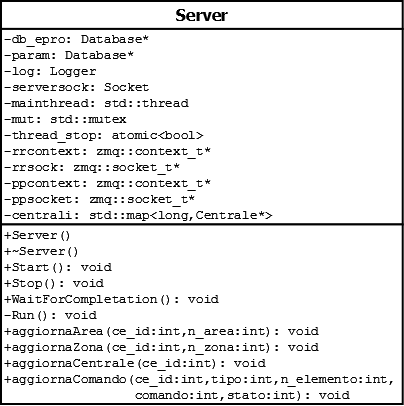
\includegraphics[width=0.5\linewidth]{pictures/serverclass.png}
	\caption{Schema della classe \texttt{Server}}\label{fig:serverclass}
\end{figure}
Il metodo \texttt{Run} della classe \texttt{Server} si occupa di gestire la comunicazione sul primo canale, esso rimane in attesa di un messaggio di richiesta, se questo messaggio è un messaggio di avvio della telegestione questo metodo crea e mette in esecuzione un'istanza di \texttt{Centrale} in base al tipo di centrale da telegestire, nel caso in cui il messaggio arrivato sia un comando il metodo \texttt{Run} ricerca la centrale all'interno della sua lista e aggiunge il comando alla sua coda di comandi; nel caso in cui il messaggio pervenuto sia di tipo “fine telegestione” questo metodo invoca il metodo \texttt{Stop} della classe \texttt{Centrale}, ne richiama il distruttore e la elimina dalla lista delle centrali. Dopo ogni operazione invia una risposta al modulo che ha inviato la richiesta.\\
Oltre ai consueti metodi di servizio già visti in tutte le classi, ovveto \texttt{Start}, \texttt{Stop} e \texttt{WaitingForCompletation} che servono a gestire il thread troviamo i metodi:
\begin{itemize}
	\item \texttt{aggiornaArea}
	\item \texttt{aggiornaZona}
	\item \texttt{aggiornaCentrale}
	\item \texttt{aggiornaComando}
\end{itemize}
Che servono per la comunicazione sul secondo canale, infatti questi quattro metodi non fanno altro che prelevare le informazioni passate come parametri interpretarle e creare il pacchetto corrispondente ed inviarlo pubblicarlo sul secondo canale di comunicazione al JBoss.
\subsubsection{GestioneRichiesteRisposte}
\begin{figure}
	\centering
	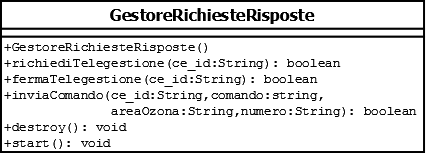
\includegraphics[width=0.5\linewidth]{pictures/classgestore.png}
	\caption{Classe \texttt{GestoreRichiesteRisposte}}\label{fig:gestricclass}
\end{figure}
Questa classe si occupa della gestione della comunicazione di tipo \emph{request-replay}, i suoi metodi vengono invocati da un livello più alto del software che noi non tratteremo.\\
Lo schema della classe è mostrato in \fname{fig:gestricclass} nel quale sono mostrati i metodi principali e non l'intera struttura della classe, tali metodi sono abbastanza facili da comprendere; il metodo \texttt{richiediTelegestione} riceve in ingresso il codice identificativo della centrale da telegestire, esso crea la connessione sul canale \emph{request-replay}, invia il comando di inizio telegestione ed attende la risposta positiva del server. Il metodo \texttt{fermaTelegestione} riceve come parametro il codice identificativo della centrale e con tale codice crea il pacchetto per fermare la telegestione, lo invia sul primo canale di comunicazione ed attende la risposta la quale sarà comunicata al livello superiore del software tramite il valore restituito dal metodo.\\
Il metodo \texttt{inviaComando} riceve come parametri di ingresso il codice identificativo della centrale, il comando da eseguire, il tipo di elemento sul quale eseguirlo e il numero dell'elemento. In particolare esso riceve i parametri direttamente nello standard del protocollo e non è quindi necessario tradurre tali dati per creare il messaggio da inviare; dopo aver preparato il pacchetto lo invia sul canale e si mette in attesa della risposta.
\subsubsection{ReceiverThread}
Questa classe si occupa della ricezione dei messaggi sul canale di trasmissione \emph{publish-subscribe}. Essa implementa un thread messo in esecuzione quando esiste almeno una sessione attiva di telegestione e si preoccupa solamente di ricevere i messaggi, non di decifrarli, essi vengono immessi in una coda la quale verrà svuotata ad un livello superiore del software nel quale verranno anche decifrati.\\
Questa classe estende la classe \texttt{Thread} e quindi non necessità dell'implementazione di altri metodi oltre al metodo \texttt{run}.
\subsection{Implementazione}
Per quanto riguarda il la classe \texttt{Server} essa è stata implementata in C++ come il resto del software Telegestore utilizzando lo standard del 2011 (ISO/IEC 14882:2011\cite{c++11}) in modo da supportare il multi-threading  in modo nativo, per fare ciò si è deciso di utilizzare il compilatore gcc-4.8, la più completa al momento in cui abbiamo sviluppato.\\
Per quanto riguarda le due classi in esecuzione sul server JBoss sono state sviluppate utilizzando il linguaggio Java aggiornato alla versione 1.5; questa scelta è stata obbligata dal resto del software in esecuzione che sfrutta dei metodi deprecati e un comportamento scorretto della stessa implementazione di Java e che quindi non può essere aggiornato. Inoltre lo stesso JBoss\cite{jboss} utilizzato non permette un aggiornamento all'ultima versione del linguaggio Java in quanto la versione utilizzata dell'application server è la 4.\\
Per quanto riguarda la camunicazione tra la classe \texttt{Server} e le due classi in esecuzione sul server JBoss è stato utilizzato il framework \emph{ZeroMQ}\cite{zmq} aggiornato alla versione 1.3 questo framework permette la creazione di diversi patern di comunicazione come il \emph{request-replay} utilizzato per il primo canale o il \emph{public-subscribe} utilizzato per il secondo senza doverci preoccupare di gestire la connessione o di controllare il corretto invio e ricezione dei messaggi.
\subsubsection{Server}
Questa classe si divide in due parti, la prima parte composta dal metodo \texttt{Run} e dai metodi che gestiscono il thread si occupa dello scambio dei messaggi sul primo canale di comunicazione, quello di tipo request-replay. Il funzionamento del metodo \texttt{Run} è molto semplice come si nota dal diagramma in \fname{fig:flussoserver}, il metodo si pone in attesa di un messaggio, in caso sia un messaggio di inizio esso invoca la creazione di una nuova istanza della classe \texttt{Centrale} e su questa istanza invoca il metodo \texttt{Start} nel caso in cui invece sia un messaggio di fine telegestione allora il metodo controlla la lista delle centrali ed elimina la centrale richiesta. Nel caso in cui, infine, il messaggio arrivato sia un messaggio di richiesta comando, allora il metodo crea un nuovo \texttt{Comando} e lo inserisce nella lista dei comandi adeguata.
\begin{figure}
\centering
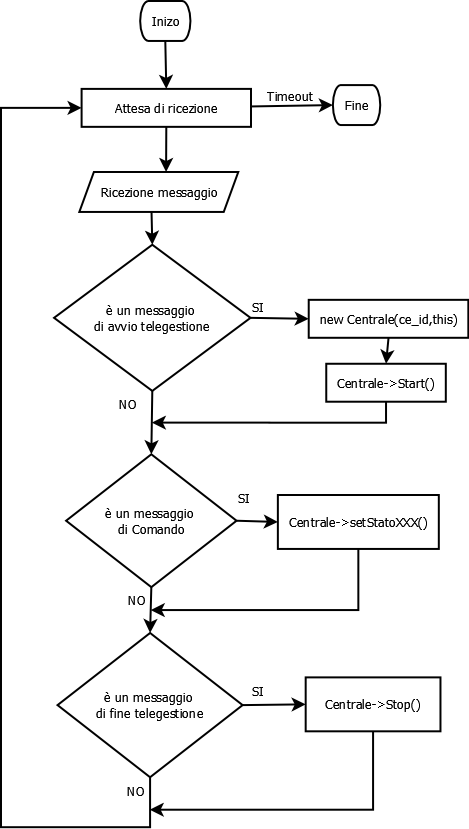
\includegraphics[width=0.7\linewidth]{pictures/flussoserver.png}
\caption{Diagramma di flusso per il metodo \texttt{Run} della classe \texttt{Server}}\label{fig:flussoserver}
\end{figure}
Per quanto riguarda la seconda parte della classe essa si occupa della trasmissione dei messaggi sul secondo canale di trasmissione ed è composta dai quattro metodi:
\begin{itemize}
	\item \texttt{aggiornaArea}
	\item \texttt{aggiornaZona}
	\item \texttt{aggiornaCentrale}
	\item \texttt{aggiornaComando}
\end{itemize}
essi hanno un comportamento molto simile tra loro e non fanno altro che utilizzare i dati passati come parametro e costrutire il pacchetto che sarà successivamente inviato sul canale publish-subscribe, come possiamo vedere dal codice mostrato in \lname{lst:aggiornacode}.
\begin{lstlisting}[language=C++,caption=Metodo aggiornaXXX,label=lst:aggiornacode]
void Server::aggiornaZona(int ce_id, int n_zona) {
    std::string risposta;
    std::map<long, Centrale *>::iterator it;
    unsigned char stato;
    it = centrali.find(ce_id);
    if(it != centrali.end()) {
        stato = it->second->getStatoZone(n_zona);
        if (stato == 0xFF) {
            risposta=std::to_string(ce_id)+";1;"+std::to_string(n_zona)+";-1;-1;-1";
        } else {
            risposta=std::to_string(ce_id)+";1;"+std::to_string(n_zona)+";"+std::to_string(stato&0x01)+";"+std::to_string(stato&0x02)+";"+std::to_string(stato&0x04);
        }
    } else {
        risposta=std::to_string(ce_id)+";1;"+std::to_string(n_zona)+";-1;-1;-1";
    }
    cout<<"Risposta: "<<risposta<<endl;
    s_sendmore(*ppsock, "005");
    s_send(*ppsock, risposta);
}
\end{lstlisting}
\subsubsection{GestoreRichiesteRisposte}
Questa classe si occupa dell'invio dei messaggi sul canale \emph{request-replay} e viene invocata da un livello superiore del software in esecuzione sul server JBoss. Essa è composta da tre metodi principali:
\begin{itemize}
	\item \texttt{richiediTelegestione}
	\item \texttt{fermaTelegestione}
	\item \texttt{inviaComando}
\end{itemize}
Questi metodi sono molto simili ed hanno lo stesso comportamento, ovvero alla loro invocazione essi stabiliscono la connessione ed invano il messaggio, dopodiché si mettono in attesa di una risposta, un esempio è il codice del metodo \texttt{fermaTelegestione} mostrato nel \lname{lst:fermatele}
\lstinputlisting[language=JAVA,caption=Metodo fermaTelegestione,label=lst:fermatele]{listati/fineTelegestione.java}
L'unica differenza si presenta nel metodo \texttt{inviaComando} il quale ha diversi parametri in ingresso tutti utilizzati per creare il pacchetto da inviare ma il comportamento del metodo rimane invariato.
\subsubsection{ReceiverThread}
Questa classe estende l'oggetto Java \texttt{Thread} per questo essa implementa il metodo \texttt{run}, in questo caso è l'unico metodo implementato oltre al costruttore. In particolare esso si occupa di ricevere il messaggio dal canale \texttt{publish-subscribe} di convertirlo in una stringa e di inserirlo in una coda che poi sarà svuotata ed analizzata ad un livello superiore del software. Il codice del metodo \texttt{run} è mostrato in \lname{lst:runpublish}.
\begin{lstlisting}[language=JAVA,caption=Metodo run,label=lst:runpublish]
public void run() {
    subscriber.connect("tcp://192.168.5.188:5556");
    String subscription = "005";
    subscriber.subscribe(subscription.getBytes());
    try {
        while (!this.isInterrupted()) {
            System.out.println("In attesa di messaggi");
            String topic = subscriber.recvStr();
            if (topic == null)
                break;
            String data = subscriber.recvStr();
            System.out.println("RICEVUTO MESSAGGIO " + data);
            TextMessage message = null;
            try {
                message = queueSession.createTextMessage();
                message.setText(data);
                queueSender.send(message);
            } catch (JMSException e) {
                e.printStackTrace();
            }
        }
    } catch (ZMQException e) {
        e.printStackTrace();
    }
}
\end{lstlisting}